\begin{figure}[H]
	\centering
	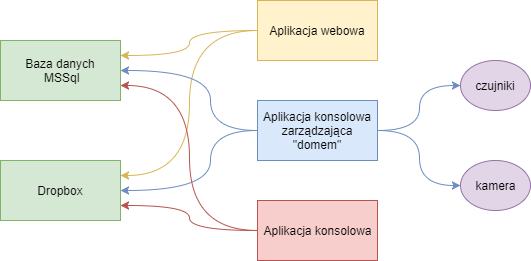
\includegraphics[scale=0.8]{schemat_systemu.png}
	\caption{Budowa systemu zarządzania domem}
	\label{fig:schemat_systemu}
\end{figure}
Aplikację powstałą na potrzeby tej pracy można podzielić na 3 moduły, które zostały przedstawione na rysunku \ref{fig:schemat_systemu}, a składają się na nie :
\begin{itemize}
\item Aplikacja webowa- interfejs pozwalający na zlecanie nowych zadań aplikacji konsolowej oraz odczyt wyników przesłanych przez nią oraz przez program zarządzający domem,
\item Aplikacja konsolowa- przetwarza zadania detekcji oraz rozpoznawania twarzy zlecone za pomocą aplikacji webowej,
\item Program zarządzający domem- przekazuje cyklicznie odczytywane dane z czujników oraz wykryte ruchy do bazy danych, w celu dalszej obróbki przez pozostałe moduły.
\end{itemize}
Na usługi pomocnicze wykorzystane w projekcie składają się
\begin{itemize}
\item baza danych- przechowywanie danych o dodanych zadaniach, wynikach, nauczonych sieciach neuronowych oraz osobach,
\item dropbox- przechowywanie większych plików- obrazów oraz nauczonych modeli sieci.
\end{itemize}

\section{Aplikacja webowa}
Aplikacja webowa jest jedyną częścią systemu, do której użytkownik może mieć bezpośredni dostęp. Strona powstała w celu maksymalnego uproszczenia procesu badania kolejnych algorytmów i usług, które różniły się sposobem podawania danych wejściowych, sposobem uczenia oraz formatem zwracanych odpowiedzi. Do pozostałych zalet takiego rozwiązania należy ułatwienie przechowywania danych, poprzez umieszczenie ich we wspólnym miejscu co pomaga, w późniejszej interpretacji wyników.
\begin{figure}[H]
	\centering
	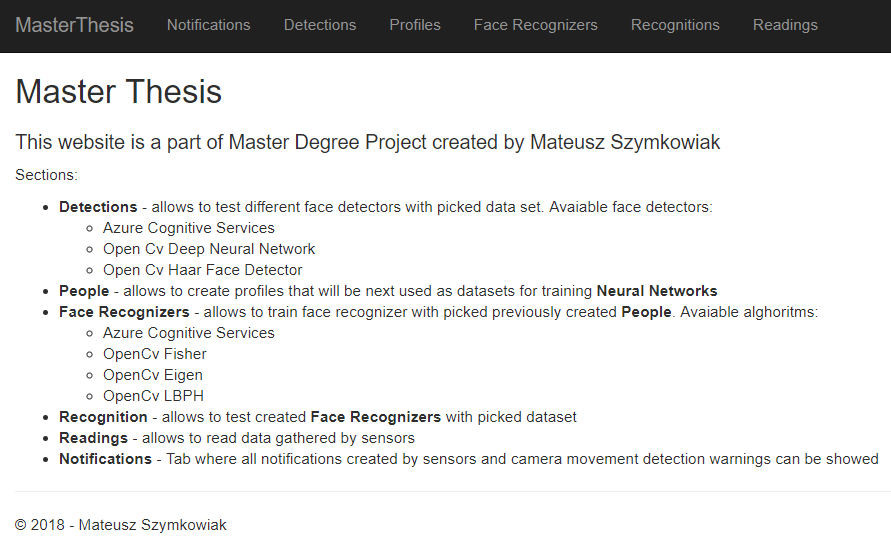
\includegraphics[scale=0.7]{aplikacja_webowa_razor_widok.png}
	\caption{Wygląd strony głównej}
	\label{fig:strona_glowna_razor}
\end{figure}
Zgodnie z interfejsem przedstawionym na rysunku \ref{fig:strona_glowna_razor}, strona została podzielona na 5 głównych sekcji:
\begin{itemize}
\item Detections- detekcje,
\item People- ludzie,
\item Neural Networks- sieci neuronowe,
\item Recognition- rozpoznawanie,
\item Sensor Readings- odczyty sensorów.
\end{itemize}
\subsection{Wzorzec projektowy MVC}
Strona internetowa powstała na bazie wzorca projektowego MVC. Założenia wzorca Model-Widok-Kontroler są bardzo proste, ich składowymi są:
\begin{itemize}
\item Model- reprezentuje logikę biznesową. Tutaj znajdują się wszelkie obiekty, które służą do wykonywania zaimplementowanej funkcjonalności danej aplikacji,
\item Widok- jest warstwą prezentacji. Odpowiada za prezentację logiki biznesowej (Modelu) użytkownikowi w przystępny sposób,
\item Kontroler- obsługuje żądania użytkownika. Odebrane zadania oddelegowuje do odpowiednich modeli.
\end{itemize}

\section{Aplikacja konsolowa}
\section{Program zarządzający domem}
